Kiến trúc vi dịch vụ có nhiều ưu điểm đặc biệt với các dự án có quy mô lớn và phức tạp.

Kiến trúc vi dịch vụ phân chia dự án thành các dịch vụ nhỏ.
Giúp việc phát triển và quản lý dễ dàng hơn.
Dễ dàng mở rộng hệ thống.
Tận dụng sử dụng tài nguyên cho từng dịch vụ.
Tập trung yêu cầu nghiệp vụ trong dịch vụ dẫn đến tốc độ định giá doanh nghiệp nhanh hơn.

Vì các dịch vụ được phân chia là độc lập.

% Nhìn chung, điều đó có nghĩa là I.T. các nhóm không cần phải đi sâu vào mọi khả năng kinh doanh. Họ có thể tập trung vào năng lực kinh doanh mà họ đang xây dựng trong vi dịch vụ của mình.

% Nhưng giả sử hoạt động kinh doanh cho vay và thế chấp đang trải qua một sự chuyển đổi nghiêm trọng nào đó, trong trường hợp đó, nhóm cho vay và thế chấp có thể quyết định phát hành vi dịch vụ của họ mỗi ngày.

Các nhóm phát triển riêng dẫn tới tốc độ phát triển thay đổi nhanh.
Giảm thiểu ràng buộc và tăng tính linh hoạt của hệ thống.
Giảm chi phí và thời gian kiểm thử do ít ràng buộc.
Hệ thống có khả năng chịu lỗi cao tăng độ tin cậy.

Kiến trúc vi dịch vụ sử dụng đa ngôn ngữ và công nghệ khác nhau.
Tận dụng hiệu quả thế mạnh của từng ngôn ngữ, công nghệ phù hợp nhất cho yêu cầu nghiệp vụ cụ thể.

Ví dụ: Mỗi dịch vụ sử dụng ngôn ngữ lập trình nhau khác như: NodeJS, Go, Python, Java, CSharp,...

\begin{figure}[h]
\centering
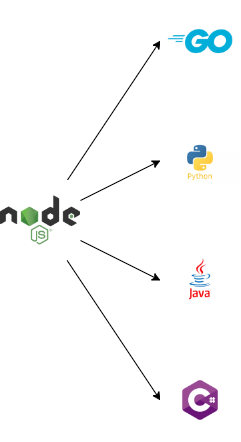
\includegraphics[height = 3cm]{pictures/DaNgonNgu/_DaNgonNgu.png}
% \caption{ViDuHinhAnhTheoChieuDoc}
\end{figure}
% Thêm vào hình SQL riêng